

The previous chapter (Ch. \ref{descY}) introduces a number of challenges for our theories of natural language semantics. Here, I provide an analysis of these phenomena, in an effort to demonstrate the utility of formal approaches to semantics and pragmatics in understanding the linguistic strategies deployed by Yolŋu Matha speakers to displace and intensionalise discourse. The analysis that follows is based on the Dhuwal language variety described above. The following chapter considers the substantial linguistic variation that occurs across the Yolŋusphere and proposes a diachronic account of the emergence of these phenomena.

The goal of this chapter (and a central aim of the dissertation) is to shed light on the meaning contributions of verbal inflections and other particles that are used in Yolŋu Matha to instantiate grammatical categories including tense, modality, polarity, aspect and evidentiality. The diagram in Figure \ref{wilk} represents an attempted schematisation of the Djambarrpuyŋu `TMA system' from Wilkinson's detailed description of the language \citeyearpar[362]{Wilkinson1991}. This diagram makes manifest the ways in which this language's inflectional semantics diverge from those of more familiar languages and underscores the difficulty of proposing a unified semantics for Yolŋu inflectional categories.

In §\ref{cycTns}, I explore the notions of ``cyclic'' and ``metrical'' tense that are manifested in a number of Yolŋu Matha varieties (as well as the unrelated non-Pama-Nyungan languages spoken elsewhere in Arnhem Land) and in §\ref{MOOD}, I consider interactions between speaker mood and felicity conditions for the verbal inflections.


	





\begin{figure}[h]\centering
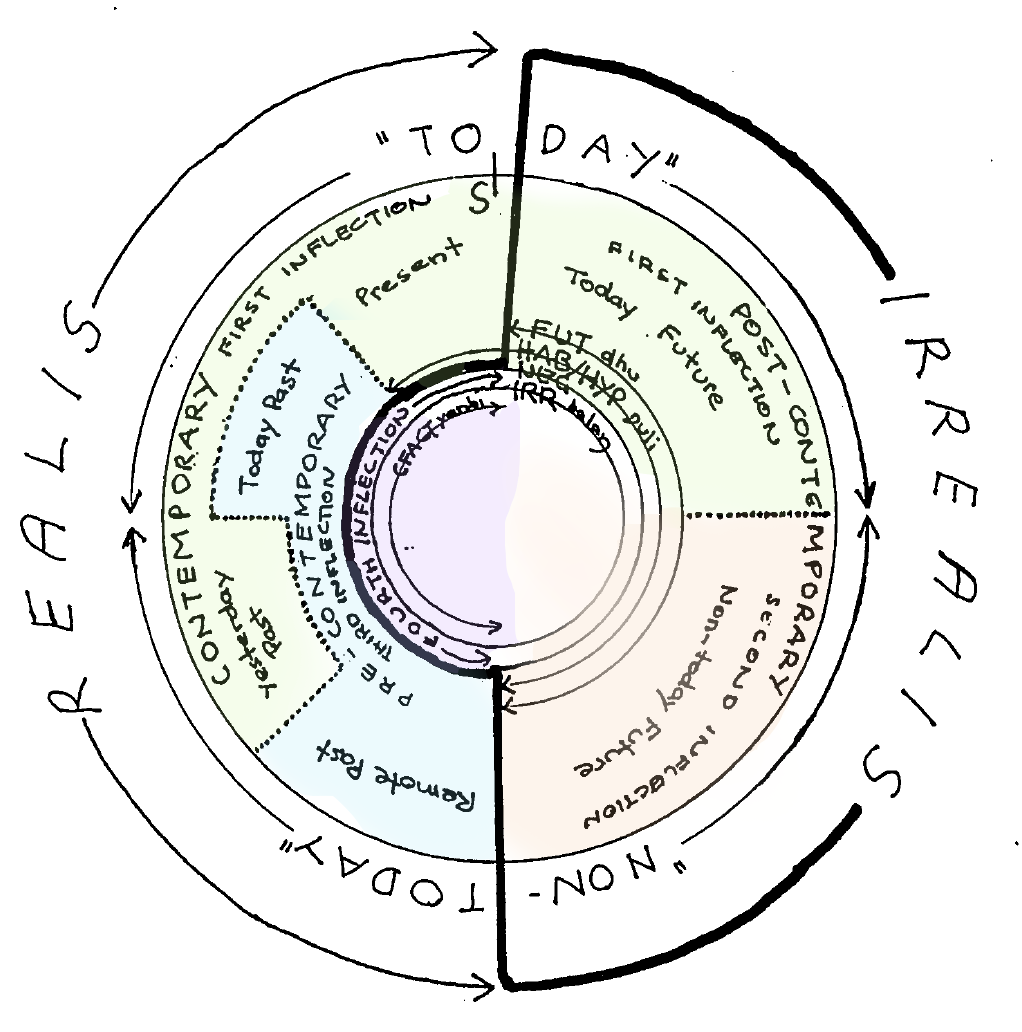
\includegraphics[width=0.75\textwidth]{WilkinsonDiagram362Col}
	\caption{Melanie Wilkinson's diagrammatic treatment of the distributional properties of Djambarrpuyŋu's four verbal inflections \citeyearpar[362]{Wilkinson1991}. Colourised by author for facilitated presentation of the `domains' of the four inflections.} \label{wilk}
\end{figure}

\section{`Cyclicity'}\label{cycTns}
\begin{quotation}
	[T]he present is like the window of a railway carriage in which we are sitting. If it were an infinitesimal slit we could not see out properly, and we could not see the countryside laid out with its features in their proper relations; but since it has a width light can enter and we can see each thing in relation to the next and so form for ourselves a picture of the whole...\hfill{\citealp[325]{Hamblin1972}}
\end{quotation}

\noindent In §\ref{infls}, I provided a description of the distributional facts of the four `inflectional classes' of Dhuwal(a). As we saw, these inflections are in a paradigmatic relation; all finite verbs receive exactly one inflection (caveat the formal identity of some of these inflections in particular verb classes (\textit{sc. }`conjugations.'))

\mcom{I think the presence of \textbf{I} here is probably just noise: speaker variation w/r/t sensitivity to the negation effect. To be confirmed.}
\begin{figure}[h]\centering\caption{Temporal expression in the Yolŋu Matha varieties of Central Arnhem, demonstrating two descriptive phenomena: (a) cyclicity --- the interspersion/discontinuity of \textbf{I} and \textbf{III} forms and (b) metricality --- the (subjective) division of the past domain between these two forms.\\$\lfloor{\sl today}\big)$ indicates the boundaries of the privileged interval {\sl today}. $\boldsymbol{t*}$ is utterance time}\label{TempSchem}
	
	
	
	\begin{tikzpicture}[scale=.85]
	% draw horizontal line   
	\draw[<->, line width=.5mm] (0,0) -- (12,0);
	
	%draw rex
	\shade[left color=blue!15!white, right color=green!15!white] (0,0.02) rectangle (4.8,1.5);
	%	\fill[green!10!white] (2.5,0.02) rectangle (4.8,1.5);
	\fill[blue!10!white] (4.8,0.02) rectangle (6.8,1.5);
	\fill[green!10!white] (6.8,0.02) rectangle (9.5,1.5);
	\fill[orange!10!white] (9.5,0.02) rectangle (12,1.5);
	
	% draw nodes
	\draw (1.25,0) node[below=3pt] {\textbf{}} node[above=10pt] {\textsc{\textbf{III}}};
	\draw (3.675,0) node[below=3pt] {\textbf{}} node[above=10pt] {\textbf{I}};
	\draw (5,0)   node[circle,fill,label=below:$\lfloor{\sl today}$] {} node[below=3pt] {\textbf{}} node[above=3pt] {};
	\draw (7,0) node[diamond,shade,outer color=black, inner color  = ochre,label=below:$\boldsymbol{t*}$] {} node[below=3pt] {\textbf{}} node[above=3pt] {\textsc{}};
	\draw (5.8,0) node[below=3pt] {\textbf{}} node[above=10pt] {\textsc{\textbf{III}}};	
	\draw (8.15,0) node[below=3pt] {\textbf{}} node[above=10pt] {\textsc{\textbf{I}}};	
	\draw (10.75,0) node[below=3pt] {\textbf{}} node[above=10pt] {\textsc{\textbf{II}}};	
	\draw (9.5,0)   node[circle,fill,label=below:${\sl today}\big)$] {} node[below=3pt] {\textbf{}} node[above=3pt] {};
	
	
	%%%braces
	
	\draw [decorate,decoration={brace,amplitude=4pt},xshift=-0pt,yshift=35pt]
	(0.5,0.5) -- (4.5,0.5) node [black,midway,yshift=0.35cm] 
	{\footnotesize metricality};
	
	\draw [decorate,decoration={brace,amplitude=4pt},xshift=-0pt,yshift=40pt]
	(3.5,0.5) -- (9,0.5) node [black,midway,yshift=0.35cm] 
	{\footnotesize cyclicity};
	
	\end{tikzpicture}\end{figure}

\section{Mood, reality status \& the speech act}\label{MOOD}

	
\begin{figure}[h]\centering\caption{Apparent interactions between temporal relations and reality status in Djambarrpuyŋu: cyclicty and metricality under negation.}
	\begin{tikzpicture}[scale=.85]
	% draw horizontal line   
	\draw[<->, line width=.5mm] (0,0) -- (12,0);
	
	%draw rex
	\shade[left color=violet!15!white, right color=orange!15!white] (0,0.02) rectangle (4.8,1.5);
	%	\fill[green!10!white] (2.5,0.02) rectangle (4.8,1.5);
	\fill[violet!10!white] (4.8,0.02) rectangle (6.8,1.5);
	\shade[left color=orange!10!white, right color=green!10!white] (6.8,0.02) rectangle (9.5,1.5);
	\fill[orange!10!white] (9.5,0.02) rectangle (12,1.5);
	
	% draw nodes
	\draw (1.25,0) node[below=3pt] {\textbf{}} node[above=10pt] {\textsc{\textbf{IV}}};
	\draw (3.675,0) node[below=3pt] {\textbf{}} node[above=10pt] {\textbf{II}};
	\draw (5,0)   node[circle,fill,label=below:$\lfloor{\sl today}$] {} node[below=3pt] {\textbf{}} node[above=3pt] {};
	\draw (7,0) node[diamond,shade,inner color=ochre,outer color=black,label=below:$\boldsymbol{t*}$] {} node[below=3pt] {\textbf{}} node[above=3pt] {\textsc{}};
	\draw (5.8,0) node[below=3pt] {\textbf{}} node[above=10pt] {\textsc{\textbf{IV}}};	
	\draw (7.5,0) node[below=3pt] {\textbf{}} node[above=10pt] {\textsc{\textbf{II}}};
	\draw (9,0) node[below=3pt] {\textbf{}} node[above=10pt] {\textsc{\textbf{I}}};	
	\draw (10.75,0) node[below=3pt] {\textbf{}} node[above=10pt] {\textsc{\textbf{II}}};	
	\draw (9.5,0)   node[circle,fill,label=below:${\sl today}\big)$] {} node[below=3pt] {\textbf{}} node[above=3pt] {};
	
	%		%braces
	%		\phantom{	\draw [decorate,decoration={brace,amplitude=4pt},xshift=-0pt,yshift=35pt]
	%			(0.5,0.5) -- (4.5,0.5) node [black,midway,yshift=0.35cm] 
	%			{\footnotesize metricality};
	%
	%			\draw [decorate,decoration={brace,amplitude=4pt},xshift=-0pt,yshift=40pt]
	%			(3.5,0.5) -- (9,0.5) node [black,midway,yshift=0.35cm] 
	%			{\footnotesize cyclicity};}
	
	\end{tikzpicture}\end{figure}
